%
% Latex comments start with the percent symbol.
%
% This file should create a pdf on a mac or Linux command line by running:
%     pdflatex hw9.tex
% I usually add a few options
%     pdflatex -halt-on-error -interaction=nonstopmode -file-line-error hw9.tex
% 
% If you are new to Latex, you might not know that you may need to run the above
% twice for the compiler to sort out its references. (There are ways to finesse
% this). 
%

\documentclass[12pt]{report}

% Whether or not you need all these packages, or even some more will vary. These
% are some common ones, but not all are needed for this document. There is no
% real harm loading your favorites out of habit. 


\usepackage{algorithm,algorithmic,alltt,amsmath,amssymb,bm,
    cancel,color,fullpage,graphicx,listings,mathrsfs,
    multirow,setspace,subcaption,upgreek,xcolor}
\usepackage[numbered,framed]{matlab-prettifier}
\usepackage[colorlinks]{hyperref}
\usepackage[nameinlink,noabbrev]{cleveref}
\usepackage[verbose]{placeins}
\usepackage{caption}
\usepackage[skip=0.1ex, belowskip=1ex,
            labelformat=brace,
            singlelinecheck=off]{subcaption}
\usepackage{float, wrapfig, multicol}

\doublespacing

%%%%%%%%%%%%%%%%%%%%%%%%%%%% Operators %%%%%%%%%%%%%%%%%%%%%%%%%%%%%%%
% Your personal shortcuts. You do not need to use any. argmax and argmin
\DeclareMathOperator*{\argmax}{arg\,max}
\DeclareMathOperator*{\argmin}{arg\,min}

%% Distributions
\newcommand{\N}{\mathcal{N}}
\newcommand{\U}{\mathcal{U}}
\newcommand{\Poi}{{\text Poisson}}
\newcommand{\Exp}{{\text Exp}}
\newcommand{\G}{\mathcal{G}}
\newcommand{\Ber}{{\text Bern}}
\newcommand{\Lap}{{\text Laplace}}
\newcommand{\btheta}{\boldsymbol{\theta}}
\newcommand{\bSigma}{\boldsymbol{\Sigma}}
% \usepackage[left=1cm,right=2.5cm,top=2cm,bottom=1.5cm]{geometry}
% Code blocks formatting

\definecolor{MyDarkGreen}{rgb}{0.0,0.4,0.0}

% For faster processing, load Matlab syntax for listings
\lstloadlanguages{Matlab}%
\lstset{language=Matlab,        % Use MATLAB
        % frame=single,   % Single frame around code
        basicstyle=\small\ttfamily,     % Use small true type font
        keywordstyle=[1]\color{blue}\bfseries,  % MATLAB functions bold and blue
        keywordstyle=[2]\color{purple}, % MATLAB function arguments purple
        keywordstyle=[3]\color{blue}\underbar,  % User functions underlined and blue
        identifierstyle=,       % Nothing special about identifiers
        % Comments small dark green courier
        commentstyle=\usefont{T1}{pcr}{m}{sl}\color{MyDarkGreen}\small,
        stringstyle=\color{purple},     % Strings are purple
        showstringspaces=false,         % Don't put marks in string spaces
        tabsize=2,      % 2 spaces per tab
        %%% Put standard MATLAB functions not included in the default language here
        morekeywords={xlim,ylim,var,alpha,factorial,poissrnd,normpdf,normcdf},
        %%% Put MATLAB function parameters here
        morekeywords=[2]{on, off, interp},
        %%% Put user defined functions here
        morekeywords=[3]{hw1,hw2,},
        gobble=4,
        morecomment=[l][\color{blue}]{...},     % Line continuation (...) like blue comment
        numbers=left,   % Line numbers on left
        firstnumber=1,          % Line numbers start with line 1
        numberstyle=\tiny\color{blue},  % Line numbers are blue
        stepnumber=5    % Line numbers go in steps of 5
}

%% Probability
\newcommand{\E}[1]{\mathbb{E}[#1]}
\newcommand{\Cov}[2]{\mathbb{C}\mathrm{ov}(#1,#2)}

%% Bold font for vectors from Ernesto, but I do not know how the first one
%  works, but it seems necessary for the second?
\def\*#1{\mathbf{#1}}
\newcommand*{\V}[1]{\mathbf{#1}}

%%%%%%%%%%%%%%%%%%%%%%%%%%%%%%%%%%%%%%%%%%%%%%%%%%%%%%%%%%%%%%%%%%%%%%

\begin{document}


\centerline{\it CS 577}
\centerline{\it HW \#9 Submission}
\centerline{\it Name: Joses Omojola}

Questions from Part A and B were completed in matlab and saved in the \emph{hw9.m} program. The program creates an \emph{output} folder to save images, so that the 
root directory is not always cluttered (it exports 28 images), and it can be run using the \textit{hw9()} command. Most of the results are exported as graphics, and 
nothing significant is printed in terminal. To run the program, I had to install \emph{vlfeat-0.9.21} manually in Matlab. Using the provided binaries and moving back and forth 
between terminal was not too convenient, and if I can do it, you probably can too (@TA). Some questions were confusing, so I had duplicate answers to try to cover all 
my bases. If you encounter multiple responses, please grade the correct one.  Many images were plotted within functions so adding descriptive titles, axis labels, and 
legends were not easy because of the high number of images exported. All image measurements are in pixels, and I described images within captions and preceding paragraphs
where necessary. Without further ado, let's start.

\begin{enumerate}

    \item[Part A.]
    \item[A1.]  For each slide-frame keypoint, I created a collage of points matched by Euclidean distance. For this question, the first sentence asked us to find the best 
    keypoint for every image pair (which can only be one value), and then goes on to request we plot a subset of N-points (multiple values) for plotting purposes. Because I 
    was confused, I created 6 plots for this question. The first 3 images from \Cref{fig:Figure1,fig:Figure2,fig:Figure3}, show only the best slide frame keypoinrs for the 
    3 image pairs, while the remaining 3 images \Cref{fig:Figure4,fig:Figure5,fig:Figure6} shows every $5^{th}$ matched keypoint across each image pair. The keypoint error 
    is calculated by estimating the shortest euclidean distance for the 2 nearest neighbors. The keypoints are plotted as a series of arrow vectors and circles according to 
    Lowe's SIFT implementation convention. His implementation assumes that the y axis points upwards and the angles are measured \textbf{counter-clockwise}. Using clockwise 
    directions gives different direction vectors hence the mention for clarity, and I spent several hours trying to figure out why my initial plot vectors were not matching 
    the ones obtained from \emph{vl\_plotframe()}. Directional vectors for both images are scaled equally, and when large, the arrows don't show clearly but they're there.

    \begin{figure}[H]
        \centering
        \includegraphics[scale=0.5]{output/f01_img1_best_eucl_dist.png}
        \caption{Best keypoint for slide1 and frame1 image pair. Directional vectors of keypoints with yellow arrows indicating scale and orientation. Yellow circles 
        show keypoint locations on the left. Coordinates of matched keypoints are shown with magenta circles and joined with the yellow line (right).}
        \label{fig:Figure1}
    \end{figure}

    \begin{figure}[H]
        \centering
        \includegraphics[scale=0.5]{output/f02_img2_best_eucl_dist.png}
        \caption{Best keypoint for slide2 and frame2 image pair. Directional vectors of keypoints with green arrows indicating scale and orientation. Green circles 
        show keypoint locations on the left. Coordinates of matched keypoints are shown with magenta circles and joined with the green line (right).}
        \label{fig:Figure2}
    \end{figure}

    \begin{figure}[H]
        \centering
        \includegraphics[scale=0.5]{output/f03_img3_best_eucl_dist.png}
        \caption{Best keypoint for slide3 and frame3 image pair. Directional vectors of keypoints with red arrows indicating scale and orientation. Red circles 
        show keypoint locations on the left. Coordinates of matched keypoints are shown with magenta circles and joined with the red line (right).}
        \label{fig:Figure3}
    \end{figure}

    \begin{figure}[H]
        \centering
        \includegraphics[scale=0.75]{output/f04_img1_eucl_dist_5N.png}
        \caption{Plot of every 5 keypoints for slide1 and frame1 image pair. Error type is euclidean distance and no filter is applied to select a percentage of 
        points. Directional vectors and matched point descriptions are same as figure 1.}
        \label{fig:Figure4}
    \end{figure}

    \begin{figure}[H]
        \centering
        \includegraphics[scale=0.75]{output/f05_img2_eucl_dist_5N.png}
        \caption{Plot of every 5 keypoints for slide2 and frame2 image pair. Error type is euclidean distance and no filter is applied to select a percentage of 
        points. Directional vectors and matched point descriptions are same as figure 2.}
        \label{fig:Figure5}
    \end{figure}

    \begin{figure}[H]
        \centering
        \includegraphics[scale=0.75]{output/f06_img3_eucl_dist_5N.png}
        \caption{Plot of every 5 keypoints for slide3 and frame3 image pair. Error type is euclidean distance and no filter is applied to select a percentage of 
        points. Directional vectors and matched point descriptions are same as figure 3.}
        \label{fig:Figure6}
    \end{figure}

    \item[A2a.] This is similar to question 1 i.e. they both utilize the Euclidean distance error with the exception that I selected the best P=20\% of the matches. After
    testing different P values below and above 20, I settled on using 20 because it provided a good blend of highlighting enough points that the plots didn't appear sparse 
    for slide2-frame2 (has the least number of matched pairs overall). P=10\% gave more accurate results but very few points. Plots for other P value tests are not shown 
    here, and a subset of N=5 points is used for related figures. Output images are shown in \Cref{fig:Figure7,fig:Figure8,fig:Figure9}. The plots are less cluttered and 
    the quality of matched points is better that what was obtained in Figure 1. The right-hand side of the powerpoint is covered by the speaker in frame2, and correspoints 
    keypoints in the slide image are incorrectly matched (\autoref{fig:Figure8}).

    \begin{figure}[H]
        \centering
        \includegraphics[scale=0.75]{output/f07_img1_top20pct_eucl_dist_5N.png}
        \caption{Plot of every 5 keypoints for slide1 and frame1 image pair. Error type is euclidean distance and points are filtered above P=20\%. Directional 
        vectors and matched point descriptions are same as figure 1.}
        \label{fig:Figure7}
    \end{figure}

    \begin{figure}[H]
        \centering
        \includegraphics[scale=0.75]{output/f08_img2_top20pct_eucl_dist_5N.png}
        \caption{Plot of every 5 keypoints for slide2 and frame2 image pair. Error type is euclidean distance and points are filtered above P=20\%. Directional 
        vectors and matched point descriptions are same as figure 2.}
        \label{fig:Figure8}
    \end{figure}

    \begin{figure}[H]
        \centering
        \includegraphics[scale=0.75]{output/f09_img3_top20pct_eucl_dist_5N.png}
        \caption{Plot of every 5 keypoints for slide3 and frame3 image pair. Error type is euclidean distance and points are filtered above P=20\%. Directional 
        vectors and matched point descriptions are same as figure 3.}
        \label{fig:Figure9}
    \end{figure}

    \item[A2b.] To show the difference in error types on matched keypoints, the \textbf{cosine} distance error was used for \Cref{fig:Figure10,fig:Figure11,fig:Figure12}.
    The number of matched keypoints was almost equivalent to the euclidean distance results, however, visual inspection shows that many of the points were incorrectly 
    matched to different parts of each image image. It wasn't easy to quantify which method was better at this point. The P value of 20, and N=5 subsets was also used for 
    this plot.

    \begin{figure}[H]
        \centering
        \includegraphics[scale=0.75]{output/f10_img1_top20pct_cosi_dist_5N.png}
        \caption{Plot of every 5 keypoints for slide1 and frame1 image pair. Error type is cosine distance and points are filtered above P=20\%. Directional 
        vectors and matched point descriptions are same as figure 1.}
        \label{fig:Figure10}
    \end{figure}

    \begin{figure}[H]
        \centering
        \includegraphics[scale=0.75]{output/f11_img2_top20pct_cosi_dist_5N.png}
        \caption{Plot of every 5 keypoints for slide2 and frame2 image pair. Error type is cosine distance and points are filtered above P=20\%. Directional 
        vectors and matched point descriptions are same as figure 2.}
        \label{fig:Figure11}
    \end{figure}

    \begin{figure}[H]
        \centering
        \includegraphics[scale=0.75]{output/f12_img3_top20pct_cosi_dist_5N.png}
        \caption{Plot of every 5 keypoints for slide3 and frame3 image pair. Error type is cosine distance and points are filtered above P=20\%. Directional 
        vectors and matched point descriptions are same as figure 3.}
        \label{fig:Figure12}
    \end{figure}

    \item[A2c.] The \textbf{chi-square $(\chi^2)$} distance error metric was used for this question. Defined as 
    \[
    \chi^2 = \frac{1}{2} \Sigma^n_{i=1} \frac{(x_i - y_i)^2}{(x_i + y_i)}
    \]
    It was passed as a custom function to matlab \emph{knnsearch()}. The resulting keypoints on the slide3-frame3 pair was very good and even better than the euclidean 
    distance result but it performed rather badly on the remaining two image pairs. The P value of 20, and N=5 subsets was also used for this question. The resulting 
    images are shown in \Cref{fig:Figure13,fig:Figure14,fig:Figure15}.

    \begin{figure}[H]
        \centering
        \includegraphics[scale=0.75]{output/f13_img1_top20pct_chsq_dist_5N.png}
        \caption{Plot of every 5 keypoints for slide1 and frame1 image pair. Error type is chi-square distance and points are filtered above P=20\%. Directional 
        vectors and matched point descriptions are same as figure 1.}
        \label{fig:Figure13}
    \end{figure}

    \begin{figure}[H]
        \centering
        \includegraphics[scale=0.75]{output/f14_img2_top20pct_chsq_dist_5N.png}
        \caption{Plot of every 5 keypoints for slide2 and frame2 image pair. Error type is chi-square distance and points are filtered above P=20\%. Directional 
        vectors and matched point descriptions are same as figure 2.}
        \label{fig:Figure14}
    \end{figure}

    \begin{figure}[H]
        \centering
        \includegraphics[scale=0.75]{output/f15_img3_top20pct_chsq_dist_5N.png}
        \caption{Plot of every 5 keypoints for slide3 and frame3 image pair. Error type is chi-square distance and points are filtered above P=20\%. Directional 
        vectors and matched point descriptions are same as figure 3.}
        \label{fig:Figure15}
    \end{figure}

    In summary, from my visual inspection, I preferred the Euclidean distance error. It didn't always give the best results, but it provided a good balance between matching 
    enough accurate keypoints and minimizing false positive matches across the 3 image pairs compared to the other error types.

    \item[A3.] I applied the Lowe's ratio on the distance measurements for the immediate neighbor and the second nearest neighbor. Using a cutoff of 0.8 worked fine 
    for my estimate, and higher thresholds started removing some correctly matched keypoints in some of my tests. At P=20\%, it was dropping too many points, so I 
    increased P=30\% for this question and set N=1. It helped to minimize the effect of incorrectly matched keypoints across the image pairs for all images. During this 
    test, it was easier to see the effect of the different error types. Euclidean distance gave the least number of matched points with the highest accuracy compared to 
    cosine and chi-square errors, which provided more keypoints with higher false-positive rates. Resulting images are shown in \Cref{fig:Figure16,fig:Figure17,fig:Figure18}.

    \begin{figure}[H]
        \centering
        \includegraphics[scale=0.75]{output/f16_img1_top30pct_eucl_dist_1N_prune.png}
        \caption{Plot of all keypoints for slide1 and frame1 image pair. Error type is Euclidean distance and points are filtered above P=30\%. A Lowe's ratio of 0.8 
        is used to filter uncorrelated points. Directional vectors and matched point descriptions are same as figure 1.}
        \label{fig:Figure16}
    \end{figure}

    \begin{figure}[H]
        \centering
        \includegraphics[scale=0.75]{output/f17_img2_top30pct_eucl_dist_1N_prune.png}
        \caption{Plot of all keypoints for slide2 and frame2 image pair. Error type is Euclidean distance and points are filtered above P=30\%. A Lowe's ratio of 0.8 
        is used to filter uncorrelated points. Directional vectors and matched point descriptions are same as figure 2.}
        \label{fig:Figure17}
    \end{figure}

    \begin{figure}[H]
        \centering
        \includegraphics[scale=0.75]{output/f18_img3_top30pct_eucl_dist_1N_prune.png}
        \caption{Plot of all keypoints for slide3 and frame3 image pair. Error type is Euclidean distance and points are filtered above P=30\%. A Lowe's ratio of 0.8 
        is used to filter uncorrelated points. Directional vectors and matched point descriptions are same as figure 3.}
        \label{fig:Figure18}
    \end{figure}

    \item[A4.] Using two nested for loops with an euclidean distance error, Lowe's ratio of 0.8, and P=1, I compared the number of matched points for all slide and image 
    pairs. The resulting confusion matrix is shown in (\autoref{fig:Figure19}). The highest correlation from the confusion matrix should be when the appropriate slide numbers 
    are matched with their corresponding video frame however, I noticed slide1 had a high number of matched points with frame2. The plotted figure of that pair is shown in 
    (\autoref{fig:Figure20}). Many background points are matched across the image pair and the algorithm might be tricked by the similar brightness on the background of 
    both images (Similar background color and contrast can influence brighness in grayscale images). Apart from this spurious pair, the remaining slides have the highest 
    keypoint matches when compared to the corresponding video frames.

    \begin{figure}[H]
        \centering
        \includegraphics[scale=0.75]{output/f20_confusion_matrix.png}
        \caption{Confusion matrix showing the number of matched keypoints for all slide-frame pairs. Slides are shown as rows, while video frames are represented as columns.}
        \label{fig:Figure19}
    \end{figure}

    \begin{figure}[H]
        \centering
        \includegraphics[scale=0.75]{output/f19_anomalous_figure.png}
        \caption{Spuriously matched keypoints for slide1 and frame2 image pair. A lot of the points from slide1 are matched to a background point on frame2.}
        \label{fig:Figure20}
    \end{figure}

    \item[Part B.]
    \item[B1.] I implemented a custom Harris corner detector function in Matlab. The function considers the $k$ value, threshold $(t)$, and gaussian $\sigma$ scale. The 
    window size is formulated as being proportional to the $\sigma$ scale, where $ws = 2(\sigma) + 1$. This is used to implement non-maximal suppression for clusters of 
    neighboring pixels around edges. The threshold is designed to be a percentage of the maximum value for the Harris response matrix $(R)$, and typically ranges between 
    0.01-0.1. Because a high-number of points are exported, I put in a flag to regulate the best-n points that should be displayed for each test. The parameters used for 
    all tests are displayed in the figure titles.  

    I tested it on a variety of images in different scenarios while tweaking the input parameters as suggested by the question. My simplest test was performed 
    using an image of a checkerboard with clearly defined edges. Increasing the gaussian smoothing kernel size, tends to offset fine edges near the boundaries of the image 
    as shown in (\autoref{fig:Figure21}). Adjusting the $K$ value below \emph{0.2} didn't have major impacts on the recovered edgepoints, but as $K$ increased above $(k>0.2)$, 
    less accurate edgepoints were resolved, and at some point, only points on the left corner of the image were highlighted (\autoref{fig:Figure22}). This occurs irrespective 
    of the input threshold and scale values.

    \begin{figure}[!ht]\centering
        \hspace*{-0.8in}
        \begin{subfigure}{0.40\textwidth}
            \includegraphics[scale=0.6]{output/checkbrd-small-scale.png}
            \caption{Using a \textbf{small} $(\sigma=2)$ scale to identify fine edges.}
            \label{fig:Figure21a}
        \end{subfigure}
    \hfil
        \begin{subfigure}{0.40\textwidth}
        \includegraphics[scale=0.6]{output/checkbrd-large-scale.png}
        \caption{Using a \textbf{large} $(\sigma=20)$ scale to identify fine edges.}
        \label{fig:Figure21b}
        \end{subfigure}
        \caption{Effect of changing $\sigma$ and window scale on small edge detection. Edgepoints are shown as red squares. Larger smoothing can offset fine edge points at 
        the boundaries of the image. Input arguments are shown in subfigure titles.}
        \label{fig:Figure21}
    \end{figure}

    \begin{figure}[H]
        \centering
        \includegraphics[scale=0.6]{output/checkbrd-large-k.png}
        \caption{Effect of large $K$ values on edgepoint detection. All points are aligned on left corner as $k>0.2$.}
        \label{fig:Figure22}
    \end{figure}

    While small smoothing scales are good for identifying fine edgepoints (\autoref{fig:Figure21a}), using small $\sigma$ values can cause detection of very small edgepoints 
    in larger images, constituting high-frequency noise (\autoref{fig:Figure23a}). With a larger smoothing scale $(\sigma=10)$, non-maximal suppression suppresses dense 
    clusters, allowing edgepoints like the edge of the overhang to be better resolved (\autoref{fig:Figure23b}). This can also be observed when it's applied on an image 
    from an outdoor city (\autoref{fig:Figure24}). Edges are better spaced out and can easily capture larger features instead of being concentrated in dense areas.

    \begin{figure}[!ht]\centering
        \hspace*{-0.8in}
        \begin{subfigure}{0.45\textwidth}
            \includegraphics[scale=0.25]{output/outdoor-small-scale.png}
            \caption{Using a \textbf{small} $(\sigma=2)$ scale to identify fine edges. This creates a dense cluster of edgepoints along the zip.}
            \label{fig:Figure23a}
        \end{subfigure}
    \hfil
        \begin{subfigure}{0.45\textwidth}
        \includegraphics[scale=0.25]{output/outdoor-large-scale.png}
        \caption{Using a \textbf{large} $(\sigma=20)$ scale to identify fine edges. Edgepoints are better spaced out and cluster of edegepoints are eliminated.}
        \label{fig:Figure23b}
        \end{subfigure}
        \caption{Effect of changing $\sigma$ and window scale on edge detection in an outdoor image. Edgepoints are shown as red squares. Input arguments are shown in 
        subfigure titles.}
        \label{fig:Figure23}
    \end{figure}

    \begin{figure}[H]
        \centering
        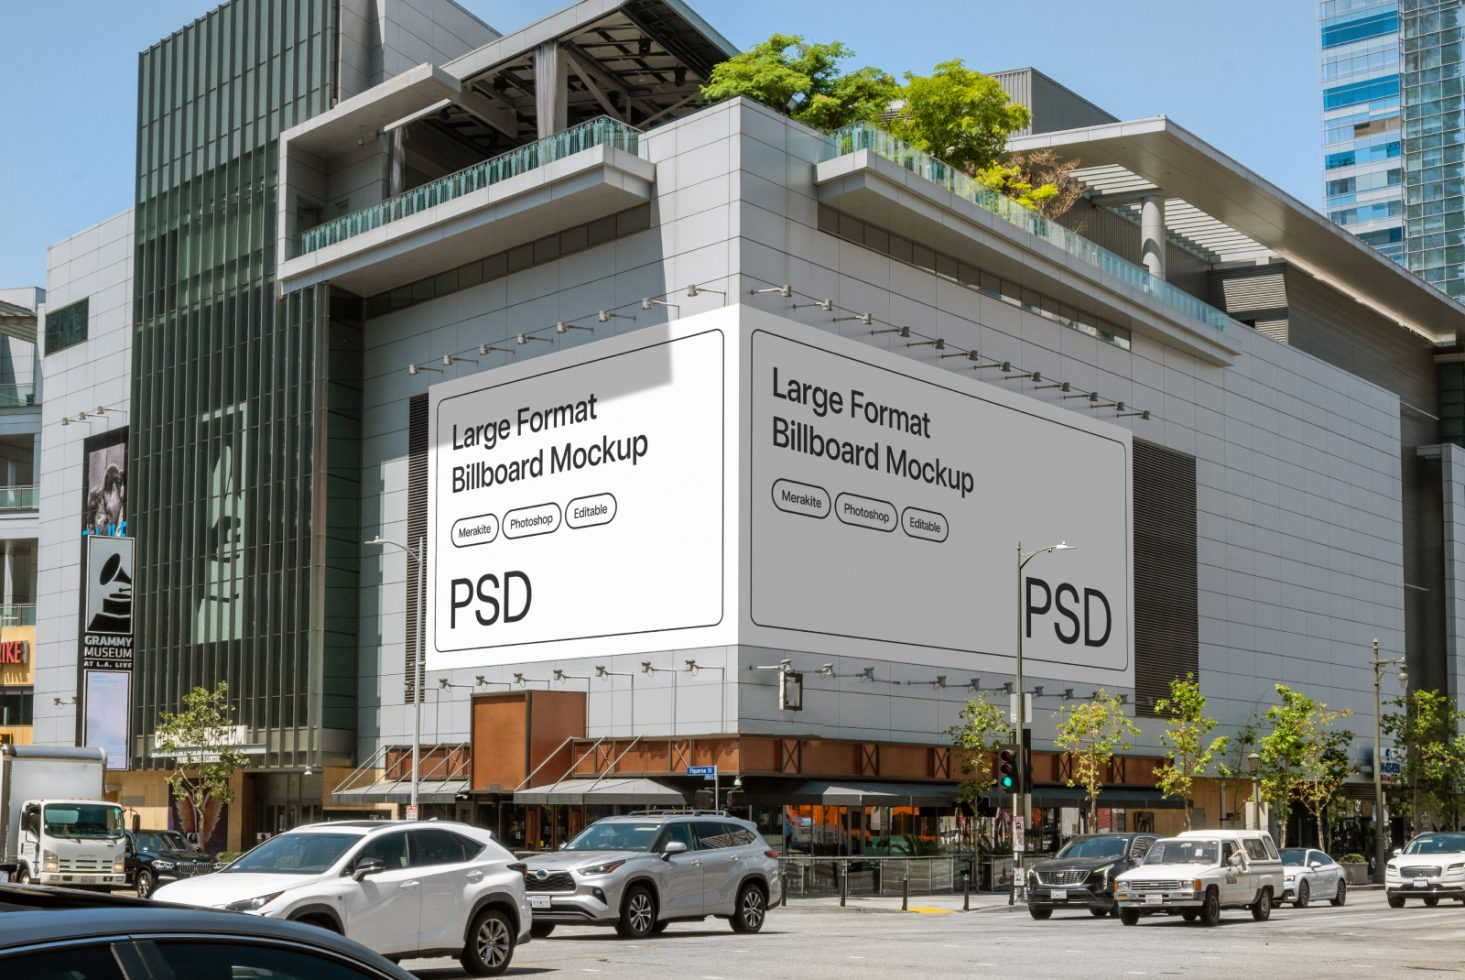
\includegraphics[scale=0.27]{output/downtown.png}
        \caption{Using larger $(\sigma=10)$ smoothing gives better spacing out of detected edgepoints at larger scales.}
        \label{fig:Figure24}
    \end{figure}

    The Harris corner detector is \textit{\textbf{rotationally invariant}}. Based on the the structure tensor \( M \) at each pixel, which is defined as:
    \[
    M = \begin{bmatrix}
    S_{I_x^2} & S_{I_x I_y} \\
    S_{I_x I_y} & S_{I_y^2}
    \end{bmatrix}
    \]
    where:\\
    - \( I_x \) and \( I_y \) are the image gradients in the \( x \)- and \( y \)-directions, respectively. \\
    - \( S_{I_x^2} \), \( S_{I_y^2} \), and \( S_{I_x I_y} \) are the products of the gradients smoothed by a Gaussian filter.  

    and the \textit{corner response} \( R \), which is computed as:
    \[
    R = \text{det}(M) - k \cdot (\text{trace}(M))^2
    \]
    where: \\
    - \( \text{det}(M) = S_{I_x^2} S_{I_y^2} - (S_{I_x I_y})^2 \) \\
    - \( \text{trace}(M) = S_{I_x^2} + S_{I_y^2} \) \\
    - \( k \) is a sensitivity parameter, typically between 0.04 and 0.06.  
    
    When the image is rotated by an angle \( \theta \), the gradients \( I_x \) and \( I_y \) transform to become:
    \[
    I_x' = I_x \cos \theta + I_y \sin \theta
    \]
    \[
    I_y' = -I_x \sin \theta + I_y \cos \theta
    \]
    The rotated gradients produce new terms \( S_{I_x'^2} \), \( S_{I_y'^2} \), and \( S_{I_x' I_y'} \), which correspond to the elements of the rotated structure 
    tensor \( M' \). The tensor transforms into:
    \[
    M' = R_\theta M R_\theta^T
    \]
    where \( R_\theta \) is the rotation matrix:
    \[
    R_\theta = \begin{bmatrix}
    \cos \theta & \sin \theta \\
    -\sin \theta & \cos \theta
    \end{bmatrix}
    \]
    This transformation changes the orientation of the matrix \( M \) but does not change its eigenvalues. Since eigenvalues represent the magnitudes of intensity changes 
    in orthogonal directions, they remain the same under rotation. Because the eigenvalues of \( M \) are invariant under rotation, both \( \text{det}(M) \) and 
    \(\text{trace}(M)\) remain unchanged, making the Harris corner detector also invariant under rotation.  

    To test this, I compared the detected edgepoints for an upright indoor image and a rotated image 
    (\autoref{fig:Figure25}). The number of detected edgepoints and their positions are mostly constant indicating that the detector in rotationally invariant.

    \begin{figure}[!ht]\centering
        \hspace*{-0.8in}
        \begin{subfigure}{0.45\textwidth}
            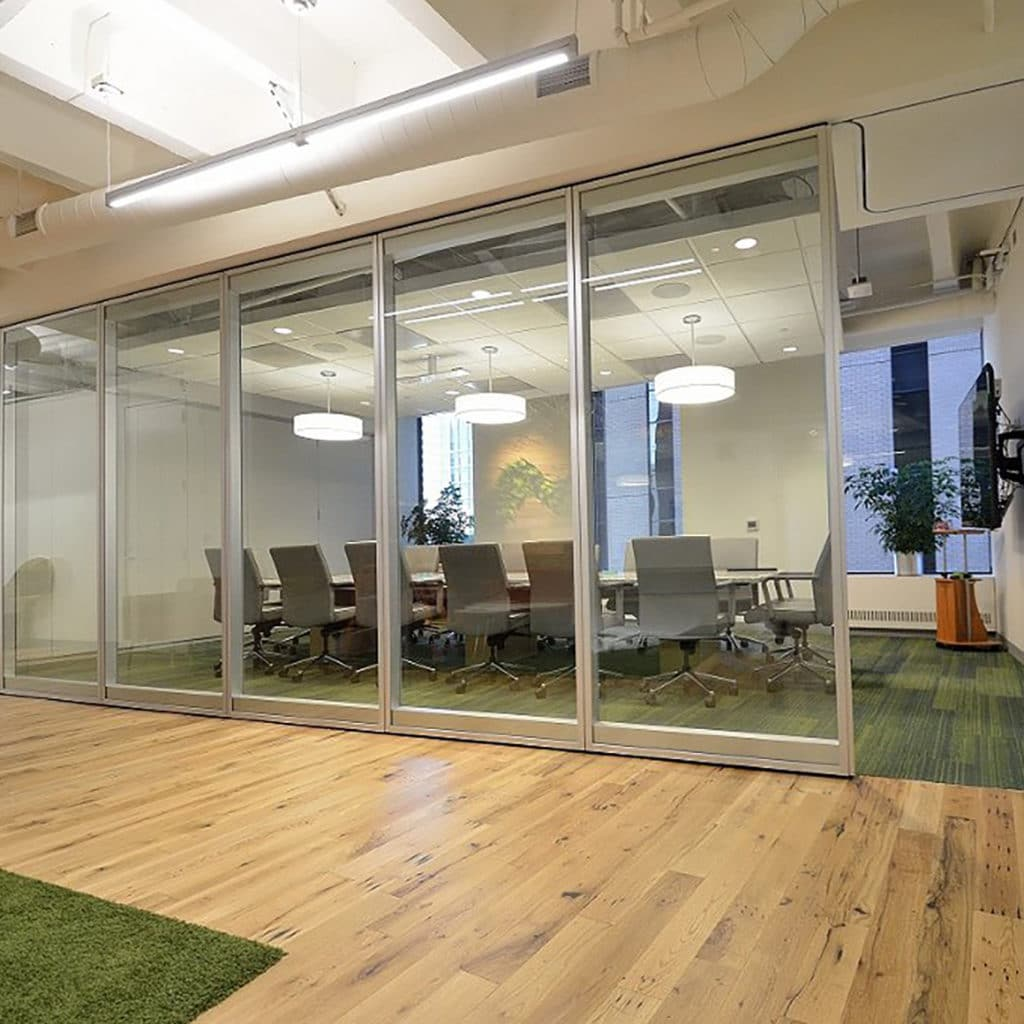
\includegraphics[scale=0.25]{output/indoor.png}
            \caption{Edge detection on upright indoor image with $(\sigma=10)$.}
            \label{fig:Figure25a}
        \end{subfigure}
    \hfil
        \begin{subfigure}{0.45\textwidth}
        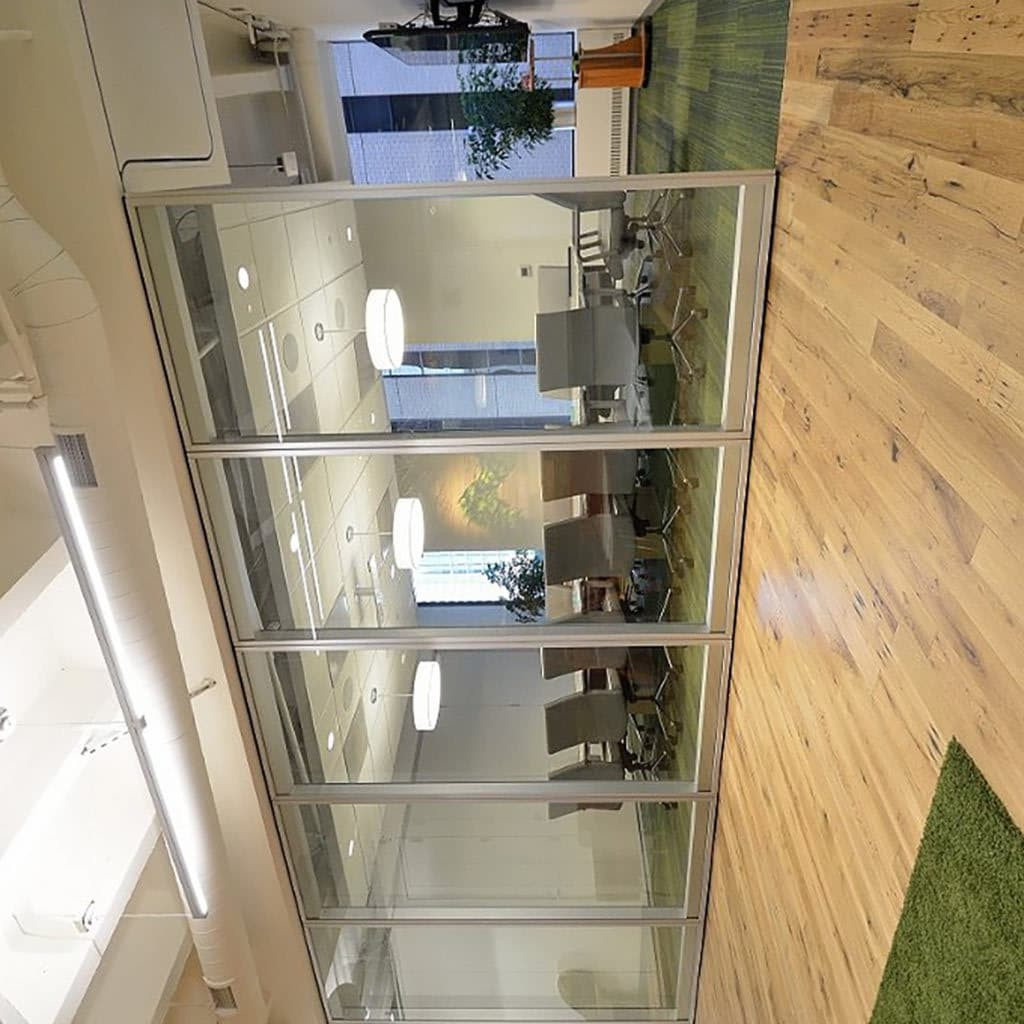
\includegraphics[scale=0.25]{output/indoor-rotate.png}
        \caption{Edge detection on rotated indoor image with $(\sigma=10)$.}
        \label{fig:Figure25b}
        \end{subfigure}
        \caption{The same number of edgepoints are detected in the upright and rotated image. Edgepoint in the top-left of both images is spurious.}
        \label{fig:Figure25}
    \end{figure}

    In summary, while the Harris detector is a good rotationally invariant edge detector, the values of the input parameters need to be tweaked to detect prominent 
    interest points at different scales, and no set of input arguments work bests across all scales. All figures to replicate report are attached in assignment submission.
\end{enumerate}

\end{document}